% Created 2016-09-03 sob 15:35
\documentclass[bigger]{beamer}
\usepackage[utf8]{inputenc}
\usepackage[T1]{fontenc}
\usepackage{fixltx2e}
\usepackage{graphicx}
\usepackage{longtable}
\usepackage{float}
\usepackage{wrapfig}
\usepackage{soul}
\usepackage{textcomp}
\usepackage{marvosym}
\usepackage{wasysym}
\usepackage{latexsym}
\usepackage{amssymb}
\usepackage{hyperref}
\tolerance=1000
\usepackage[dvipsnames]{color} 
\mode<beamer>{\usetheme{Hannover}}
\providecommand{\alert}[1]{\textbf{#1}}

\title{R programming language: conceptual overview}
\author{Maxim Litvak}
\date{2016-06-10}
\hypersetup{
  pdfkeywords={},
  pdfsubject={},
  pdfcreator={Emacs Org-mode version 7.9.3f}}

\begin{document}

\maketitle

\begin{frame}
\frametitle{Outline}
\setcounter{tocdepth}{3}
\tableofcontents
\end{frame}
\section{Introduction}
\label{sec-1}
\begin{frame}
\frametitle{R description}
\label{sec-1-1}

R is a \textbf{dynamic} language for \textbf{statistical computing} that combines \textbf{lazy functional} features and \textbf{object-oriented programming}.
\end{frame}
\begin{frame}
\frametitle{R Properties}
\label{sec-1-2}

Properties:
\begin{itemize}

\item Dynamic
\label{sec-1-2-1}%

\item Statistical computing
\label{sec-1-2-2}%

\item Lazy functional
\label{sec-1-2-3}%

\item OOP\\
\label{sec-1-2-4}%
\ldots{} R users usually focus on statistical computing, however, understanding the rest is crucial to boost productivity.
\end{itemize} % ends low level
\end{frame}
\section{Statistical computing}
\label{sec-2}
\begin{frame}
\frametitle{Statistical computing}
\label{sec-2-1}
\begin{itemize}

\item You already know how it works :-)
\label{sec-2-1-1}%
\end{itemize} % ends low level
\end{frame}
\section{Functional programming}
\label{sec-3}
\begin{frame}
\frametitle{Functional - Basics I}
\label{sec-3-1}
\begin{itemize}

\item Functional programming (FP) is a paradigm that prescribes to break down the task into evaluation of (mathematical) functions
\label{sec-3-1-1}%

\item FP is not about organizing code in subroutines (also called ``functions'' but in different sense)! (this is called procedural programming)
\label{sec-3-1-2}%

\item It's about organizing the whole programm as function
\label{sec-3-1-3}%
\end{itemize} % ends low level
\end{frame}
\begin{frame}
\frametitle{Functional - Basics II}
\label{sec-3-2}
\begin{itemize}

\item Functions as first-class objects
\label{sec-3-2-1}%
\begin{itemize}

\item can be passed as an argument
\label{sec-3-2-1-1}%

\item returned from a function
\label{sec-3-2-1-2}%

\item assigned to a variable
\label{sec-3-2-1-3}%
\end{itemize} % ends low level

\item Think of examples to the points above!
\label{sec-3-2-2}%
\end{itemize} % ends low level
\end{frame}
\begin{frame}
\frametitle{Functional - Scoping}
\label{sec-3-3}
\end{frame}
\begin{frame}[fragile]
\frametitle{Functional - Lazy}
\label{sec-3-4}
\begin{itemize}

\item ``lazy'' (or ``call-by-need'') means evaluation is delayed until value is needed
\label{sec-3-4-1}%

\item What do you think will the following piece of code work?\\
\label{sec-3-4-2}%
\begin{verbatim}
> f <- function(){g()}
\end{verbatim}


\end{itemize} % ends low level
\end{frame}
\begin{frame}[fragile]
\frametitle{Functional - Lazy}
\label{sec-3-5}
\begin{itemize}

\item It's valid even though we use function g() which isn't defined
\label{sec-3-5-1}%

\item We kind of ``promise'' that it's gonna be defined to the time than f is called
\label{sec-3-5-2}%

\item \ldots{} but if we don't keep our promise\\
\label{sec-3-5-3}%
\begin{verbatim}
> f()
Error in f() : could not find function "g"
\end{verbatim}


\end{itemize} % ends low level
\end{frame}
\begin{frame}[fragile]
\frametitle{Functional - Lazy}
\label{sec-3-6}
\begin{itemize}

\item Now, let's define the function g() before calling the function f()\\
\label{sec-3-6-1}%
\begin{verbatim}
> g <- function() 0 # now g() is defined
> f()
[1] 0
\end{verbatim}



\item Now it works
\label{sec-3-6-2}%
\end{itemize} % ends low level
\end{frame}
\begin{frame}
\frametitle{Function - Referential transparency I}
\label{sec-3-7}
\begin{itemize}

\item Referential transparency - if an expression can be replaced with its value without changing the behaviour of the program (side effect)
\label{sec-3-7-1}%

\item In R it's up to the developer, she/he should be however conscious if their code produce side effects
\label{sec-3-7-2}%

\item Assume function \textbf{g} returns 0 and function \textbf{f} returns the only argument (f <- function(x) x). Is there a difference between
\label{sec-3-7-3}%
\begin{itemize}

\item f(0)
\label{sec-3-7-3-1}%

\item f(g())
\label{sec-3-7-3-2}%
\end{itemize} % ends low level
\end{itemize} % ends low level
\end{frame}
\begin{frame}
\frametitle{Function - Referential transparency IIa}
\label{sec-3-8}
\begin{itemize}

\item Which of the following 2 cases are referential transparent?
\label{sec-3-8-1}%
\end{itemize} % ends low level
\end{frame}
\begin{frame}[fragile]
\frametitle{Function - Referential transparency IIb}
\label{sec-3-9}
\begin{itemize}

\item (cont.)
\label{sec-3-9-1}%
\begin{itemize}

\item I\\
\label{sec-3-9-1-1}%
\begin{verbatim}
> executed <- FALSE
> g <- function(){
        executed <<- TRUE
        return(0)
        }
> f(g())
\end{verbatim}



\item II\\
\label{sec-3-9-1-2}%
\begin{verbatim}
> executed <- TRUE
> g <- function(){
        executed <- FALSE
        return(0)
        }
> f(g())
\end{verbatim}


\end{itemize} % ends low level
\end{itemize} % ends low level
\end{frame}
\section{Dynamic}
\label{sec-4}
\begin{frame}[fragile,t]
\frametitle{Dynamic: Typing - I}
\label{sec-4-1}
\begin{itemize}

\item Types are optional and could be changed
\label{sec-4-1-1}%
\end{itemize} % ends low level
\begin{columns}
\begin{column}{0.6\textwidth}
\begin{block}{Code}
\label{sec-4-1-2}


\begin{verbatim}
> var <- FALSE
> class(var)
[1] "logical"
> var
[1] FALSE
> var[3] <- 1
> class(var)
"numeric"
> var
[1] 0 NA 1
\end{verbatim}
\end{block}
\end{column}
\end{columns}
\end{frame}
\begin{frame}[fragile]
\frametitle{Dynamic: Typing - II}
\label{sec-4-2}
\begin{itemize}

\item What do you think would be the type of ``var'' variable after the following action?\\
\label{sec-4-2-1}%
\begin{verbatim}
> var <- "!"
> var[3] <- 1
\end{verbatim}


\end{itemize} % ends low level
\end{frame}
\begin{frame}
\frametitle{Dynamic: Typing - III}
\label{sec-4-3}
\begin{itemize}

\item Types are implicitly there (assigned by compiler)
\label{sec-4-3-1}%

\item Types could be changed (implicitly by compiler)
\label{sec-4-3-2}%
\end{itemize} % ends low level
\end{frame}
\begin{frame}
\frametitle{Dynamic: Evaluation (Language abstraction)}
\label{sec-4-4}
\begin{itemize}

\item With ``eval'' you can dynamically evaluate code, e.g.\\
\label{sec-4-4-1}%
> eval(parse=text(``f <- function(x) x''))

\item It allows to have more freedom in code manipulation (example will follow), beware performance!
\label{sec-4-4-2}%

\item R allows to ``abstract'' the language itself
\label{sec-4-4-3}%
\end{itemize} % ends low level
\end{frame}
\section{OOP}
\label{sec-5}
\begin{frame}
\frametitle{OOP - Basics}
\label{sec-5-1}
\begin{itemize}

\item Object-oriented programming is a paradigm in programming that prescribes to break down the task into objects with particular behaviour and data.
\label{sec-5-1-1}%
\end{itemize} % ends low level
\end{frame}
\begin{frame}
\frametitle{OOP in R}
\label{sec-5-2}
\begin{itemize}

\item Competing OOP standards in R: S3 (old), S4 (newer), reference classes, special libraries (R6, proto)
\label{sec-5-2-1}%

\item xkcd:\\
\label{sec-5-2-2}%
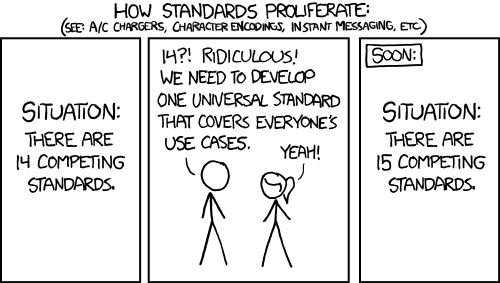
\includegraphics[width=.9\linewidth]{./standards.png}
\end{itemize} % ends low level
\end{frame}
\begin{frame}
\frametitle{OOP in R: S4}
\label{sec-5-3}
\begin{itemize}

\item Assume an object of class ``Company'' has 2 properties: headcount (HC) and earnings (EBIT)
\label{sec-5-3-1}%

\item if you ``add'' (i.e. merge) 2 companies, then you add up their earnings +20\% (synergy effects) and add up their headcount -20\% (economies of scale)
\label{sec-5-3-2}%
\end{itemize} % ends low level
\end{frame}
\begin{frame}[fragile]
\frametitle{OOP in R: S4}
\label{sec-5-4}
\begin{itemize}

\item Solution\\
\label{sec-5-4-1}%
\begin{verbatim}
> setClass("Company"
        , representation(HC = "numeric"
                , EBIT = "numeric")
)

> setMethod("+"
        , signature("Company", "Company")
        , function(e1, e2){
    new("Company"
        , HC = (e1@HC + e2@HC)*0.8
        , EBIT = (e1@EBIT + e2@EBIT)*1.2
        )
})
> Microsoft <- new("Company"
        , HC = 50, EBIT = 95)
> LinkedIn<-new("Company", HC = 2, EBIT = 5)
\end{verbatim}


\end{itemize} % ends low level
\end{frame}
\begin{frame}[fragile]
\frametitle{OOP in R: S4}
\label{sec-5-5}
\begin{itemize}

\item Result\\
\label{sec-5-5-1}%
\begin{verbatim}
> Microsoft + LinkedIn
An object of class "Company"
Slot "HC":
[1] 41.6

Slot "EBIT":
[1] 120
\end{verbatim}


\end{itemize} % ends low level
\end{frame}
\begin{frame}[fragile]
\frametitle{Comparison to other languages}
\label{sec-5-6}
\begin{itemize}

\item Python\\
\label{sec-5-6-1}%
\begin{verbatim}
class Company():
  def __init__(self, HC, EBIT):
    self.HC = HC
    self.EBIT = EBIT
  def __add__(self, other):
    return Company((self.HC+other.HC)*0.8 
        ,(self.EBIT + other.EBIT)*1.2)
  def __repr__(self):
    out="HC:%s,EBIT:%s"%(self.HC,self.EBIT)
    return out

>>> Microsoft = Company(50, 95)
>>> LinkedIn = Company(2, 5)
>>> Microsoft + LinkedIn #HC:41.6,EBIT:120.0
\end{verbatim}


\end{itemize} % ends low level
\end{frame}
\begin{frame}[fragile]
\frametitle{Comparison to other languages}
\label{sec-5-7}


\begin{verbatim}
class Company
{
  private double HC;
  private double EBIT;
  public Company(double HC, double EBIT)
  {this.HC = HC;this.EBIT = EBIT;}
  public static operator +(Company A
                        , Company B)
  {
    double HC = (A.HC + B.HC)*0.8;
    double EBIT = (A.EBIT + B.EBIT)*1.2;
    return new Company(HC, EBIT)
  }
}
\end{verbatim}
\end{frame}
\section{Statistical computing - revision I}
\label{sec-6}
\begin{frame}
\frametitle{Statistical computing - revision}
\label{sec-6-1}
\begin{itemize}

\item Example: given X (e.g. ``norm'') distribution
\label{sec-6-1-1}%
\begin{itemize}

\item pX is its probability function
\label{sec-6-1-1-1}%

\item dX is its density function
\label{sec-6-1-1-2}%

\item qX is its quantile function
\label{sec-6-1-1-3}%
\end{itemize} % ends low level

\item How to abstract X?
\label{sec-6-1-2}%

\item Construct a function that takes name of the distribution with 2 parameters as an argument (e.g. ``norm'', ``unif'') and returns its quantile function parametrized with [0;1] (hint: use ``eval'')
\label{sec-6-1-3}%
\end{itemize} % ends low level
\end{frame}
\section{Statistical computing - revision II}
\label{sec-7}
\begin{frame}[fragile]
\frametitle{Possible solution}
\label{sec-7-1}
\begin{itemize}

\item 1-st step: how could it look for a particular function\\
\label{sec-7-1-1}%
eval(parse(text=''function(x) qnorm(x,0,1)''))

\item 2-nd step: separate distribution parameter\\
\label{sec-7-1-2}%
\begin{verbatim}
eval(
  parse(
    text=paste0(
      "function(x) q","norm","(x,0,1)"
        )
    )
)
\end{verbatim}

\begin{verbatim}
 function (x) 
 qnorm(x, 0, 1)
\end{verbatim}

\end{itemize} % ends low level
\end{frame}
\section{Statistical computing - revision III}
\label{sec-8}
\begin{frame}[fragile]
\frametitle{Possible solution (cont.)}
\label{sec-8-1}
\begin{itemize}

\item 3-rd step: abstract distribution as an argument and return as function\\
\label{sec-8-1-1}%
\begin{verbatim}
F <- function(dist){
  eval(parse(
    text=paste0(
      "function(x) q", dist ,"(x,0,1)"
    )
))
}
\end{verbatim}



\item Now you can get quantiles for different distributions
\label{sec-8-1-2}%
\begin{itemize}

\item Log-normal\\
\label{sec-8-1-2-1}%
> F(``lnorm'')(0.5)
``1''

\item Uniform\\
\label{sec-8-1-2-2}%
> F(``unif'')(0.8)
``0.8
\end{itemize} % ends low level
\end{itemize} % ends low level
\end{frame}
\section{Statistical computing - revision IV}
\label{sec-9}
\begin{frame}
\frametitle{Last remark}
\label{sec-9-1}
\begin{itemize}

\item Further it can be generalize to distributions with different number of parameters and pass parameters as an argument
\label{sec-9-1-1}%
\end{itemize} % ends low level
\end{frame}
\section{Appendix}
\label{sec-10}
\begin{frame}
\frametitle{References}
\label{sec-10-1}
\begin{itemize}

\item Morandat, Floréal, et al. ``Evaluating the design of the R language.'' ECOOP 2012–Object-oriented programming. Springer Berlin Heidelberg, 2012. 104-131.
\label{sec-10-1-1}%
\end{itemize} % ends low level
\end{frame}
\begin{frame}
\frametitle{Repository}
\label{sec-10-2}
\begin{itemize}

\item You can find the latest version of this presentation here:
\label{sec-10-2-1}%

\item \hyperref[github.com-maxlit-workshops-tree-master-R-r-advanced-overview]{github.com/maxlit/workshops/tree/master/R/r-advanced-overview}
\label{sec-10-2-2}%

\end{itemize} % ends low level
\end{frame}

\end{document}
